\documentclass[12pt]{report}
\usepackage[utf8]{inputenc}
\usepackage[russian]{babel}
%\usepackage[14pt]{extsizes}
\usepackage{listings}
\usepackage{graphicx}
\usepackage{amsmath,amsfonts,amssymb,amsthm,mathtools} 
\usepackage{float}

% Для листинга кода:
\lstset{ %
language=C++,                 % выбор языка для подсветки (здесь это С)
basicstyle=\small\sffamily, % размер и начертание шрифта для подсветки кода
numbers=left,               % где поставить нумерацию строк (слева\справа)
numberstyle=\tiny,           % размер шрифта для номеров строк
stepnumber=1,                   % размер шага между двумя номерами строк
numbersep=5pt,                % как далеко отстоят номера строк от подсвечиваемого кода
showspaces=false,            % показывать или нет пробелы специальными отступами
showstringspaces=false,      % показывать или нет пробелы в строках
showtabs=false,             % показывать или нет табуляцию в строках
frame=single,              % рисовать рамку вокруг кода
tabsize=2,                 % размер табуляции по умолчанию равен 2 пробелам
captionpos=t,              % позиция заголовка вверху [t] или внизу [b] 
breaklines=true,           % автоматически переносить строки (да\нет)
breakatwhitespace=false, % переносить строки только если есть пробел
escapeinside={\#*}{*)}   % если нужно добавить комментарии в коде
}

% Для измененных титулов глав:
\usepackage{titlesec, blindtext, color} % подключаем нужные пакеты
\definecolor{gray75}{gray}{0.75} % определяем цвет
\newcommand{\hsp}{\hspace{20pt}} % длина линии в 20pt
% titleformat определяет стиль
\titleformat{\chapter}[hang]{\Huge\bfseries}{\thechapter\hsp\textcolor{gray75}{|}\hsp}{0pt}{\Huge\bfseries}


% plot
\usepackage{pgfplots}
\usepackage{filecontents}
\usetikzlibrary{datavisualization}
\usetikzlibrary{datavisualization.formats.functions}
\begin{filecontents}{LevR.dat}
100 45504
200 344852
300 1626090
400 4410053
500 8809530
600 15523926
700 27314819
800 36896674
900 151438792
1000 253111941
\end{filecontents}

\begin{filecontents}{LevT.dat}
100 50613
200 254889
300 1164803
400 3277843
500 6466829
600 10441740
700 20235150
800 27982176
900 115139281
1000 199701561
\end{filecontents}

\begin{filecontents}{DamLevR.dat}
100 22663
200 189215
300 937882
400 2605948
500 5077237
600 9041331
700 15047492
800 20829956
900 85256627
1000 158414218
\end{filecontents}



\begin{filecontents}{LevR1.dat}
101 45393
201 386372
301 1557256
401 4538718
501 9009942
601 15214595
701 26603522
801 37648086
901 139235577
1001 278285719
\end{filecontents}

\begin{filecontents}{LevT1.dat}
101 35265
201 364594
301 1113414
401 3314034
501 6511456
601 11947585
701 20274021
801 26844301
901 136919210
1001 212082553
\end{filecontents}

\begin{filecontents}{DamLevR1.dat}
101 38152
201 196174
301 919775
401 2652528
501 5171817
601 10328122
701 15001586
801 20867237
901 108043316
1001 165932409
\end{filecontents}



\begin{document}
%\def\chaptername{} % убирает "Глава"
\begin{titlepage}
	\centering
	{\scshape\LARGE МГТУ им. Баумана \par}
	\vspace{3cm}
	{\scshape\Large Лабораторная работа №5\par}
	\vspace{0.5cm}	
	{\scshape\Large По курсу: "Анализ алгоритмов"\par}
	\vspace{1.5cm}
	{\huge\bfseries Муравьиные алгоритмы\par}
	\vspace{2cm}
	\Large Работу выполнила: Лаврова Анастасия, ИУ7-55Б\par
	\vspace{0.5cm}
	\LargeПреподаватели:  Волкова Л.Л., Строганов Ю.В.\par

	\vfill
	\large \textit {Москва, 2019} \par
\end{titlepage}

\tableofcontents

\newpage
\chapter*{Введение}
\addcontentsline{toc}{chapter}{Введение}
Муравьиный алгоритм — один из эффективных полиномиальных алгоритмов для нахождения приближённых решений задачи коммивояжёра, а также решения аналогичных задач поиска маршрутов на графах. Суть подхода заключается в анализе и использовании модели поведения муравьёв, ищущих пути от колонии к источнику питания, и представляет собой метаэвристическую оптимизацию.\\

Целью данной лабораторной работы является изучение муравьиного алгоритма для решения задачи коммивояжера, анализ влияния параметров алгоритма на время его выполнения. \\

Задача: провести сравнение муравьиного алгоритма и полного перебора.\\

\chapter{Аналитическая часть}

Муравьиные алгоритмы представляют собой вероятностную жадную эвристику, где вероятности устанавливаются, исходя из информации о 
качестве решения, полученной их предыдущих решений. Они могут использоваться как для статических, так и для динамических комбинаторных оптимизационных задач. Сходимость гарантирована, то есть в любом случае мы получим оптимальное решение, однако скорость сходимости неизвестна.   \\

Идея муравьиного алгоритма - моделирование поведения муравьев, связанного с их способностью быстро находить кратчайший путь. При своем движении муравей метит путь феромоном, и эта информация используется другими муравьями для выбора пути. Это элементарное правило поведения и определяет способность муравьев находить новый путь, если старый оказывается недоступным. Рассмотрим случай, показанный на рисунке, когда на оптимальном доселе пути возникает преграда. В этом случае необходимо определение нового оптимального пути. Дойдя до преграды, муравьи с равной вероятностью будут обходить её справа и слева. То же самое будет происходить и на обратной стороне преграды. Однако, те муравьи, которые случайно выберут кратчайший путь, будут быстрее его проходить, и за несколько передвижений он будет более обогащен феромоном. Поскольку движение муравьев определяется концентрацией феромона, то следующие будут прдпочитать именно этот путь, продолжая обогощать его феромоном до тех пор, пока этот путь по какой-либо причине не станет недоступен. \\
	\begin{figure}[h]
        	\begin{center}
        		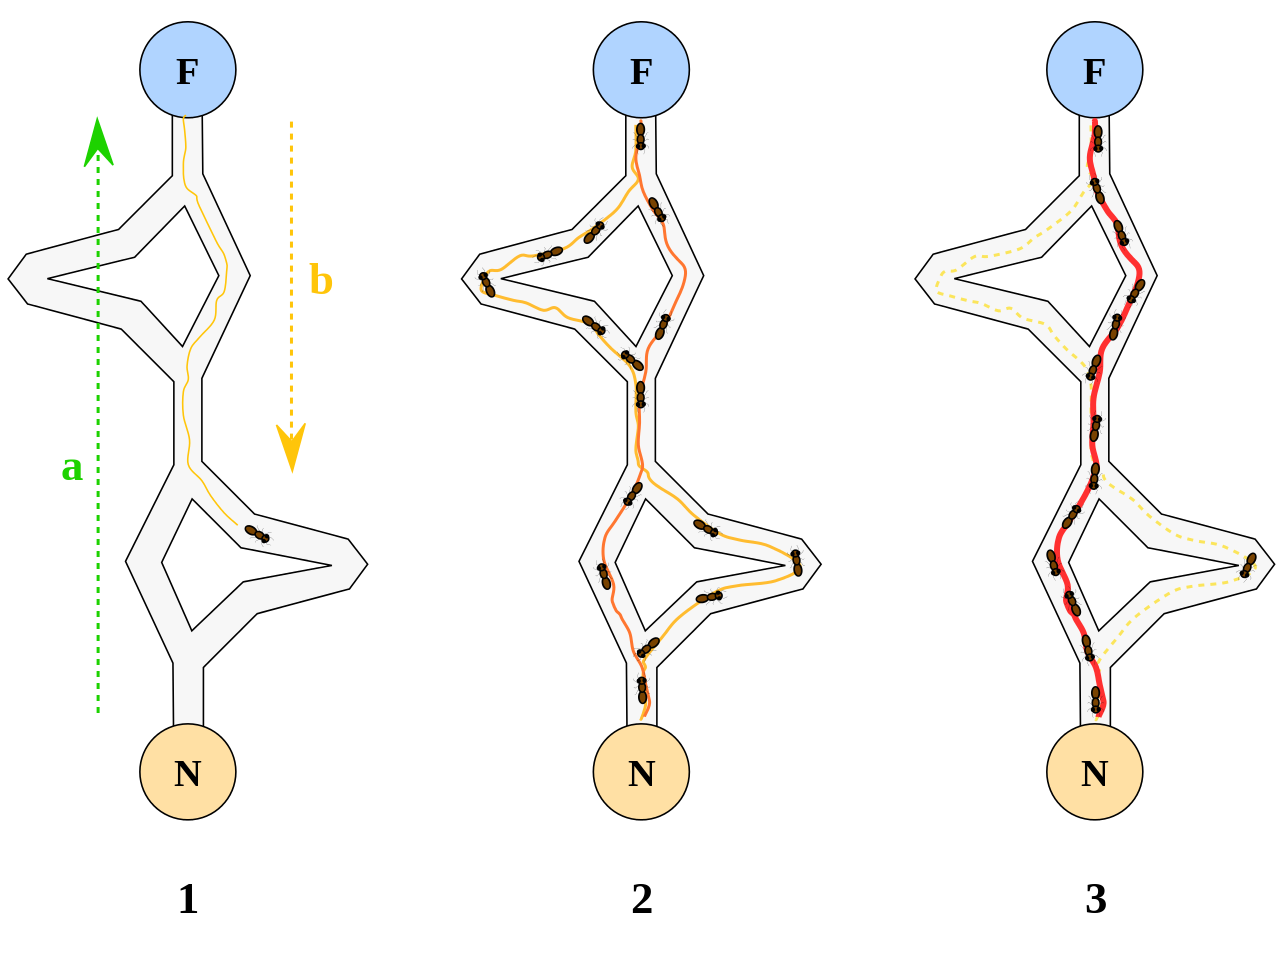
\includegraphics[scale=0.2]{ant_alg}
        		\caption{Принцип работы муравьиного алгоритма}
        		\label{fig:def}
        	\end{center}
        \end{figure}
        
Очевидная положительная обратная связь приведет к тому, что кратчайший путь станет единственным маршрутом движения большинства муравьев. Моделирование испарения феромона - отрицательной обратной связи - гарантирует нам, что найденное локально оптимальное решение не будет единственным - муравьи будут искать и другие пути. Если мы моделируем процесс такого поведения на некотором графе, рёбра которого представляют собой возможные пути перемещения муравьёв, в течение определённого времени, то наиболее обогащённый феромоном путь по рёбрам этого графа и будет являться решением задачи, полученным с помощью муравьиного алгоритма. 


\section{Обобщенный алгоритм}
Любой муравьиный алгоритм, независимо от модификаций, представим в следующем виде:
\begin{itemize}
	\item Создаем муравьев 
	\item Ищем решения 
	\item Обновляем феромон
	\item Дополнительные действия (опционально) 
\end{itemize}




\section{Применение для задачи коммивояжёра}
Теперь рассмотрим каждый шаг в цикле более подробно:\\

1. Создаем муравьёв\\
   Стартовая точка, куда помещается муравей, зависит ограничений,   накладываемых условиями задачи. Потому что для каждой задачи   способ размещения муравьёв является определяющим. Либо все    они помещаются в одну точку, либо в разные с повторения, либо    без повторений. \\
  На этом же этапе задается начальный уровень феромона. Он    инициализируется небольшим положительным числом для того,    чтобы на начальном шаге вероятности перехода в следующую    вершину не были нулевыми. \\
  
2. Ищем решения  \\
 Вероятность перехода из вершины i в вершину j определяется по следующей формуле:\\   
\begin{equation}
P_{i j, k} (t)= \begin{cases}
\displaystyle[\tau_{ij}(t)]^\alpha \cdot [\eta_{ij}]^\beta\over 
\displaystyle\sum\limits_{l \in J_{i, k }} [\tau_{il}(t)]^\alpha \cdot \eta_{il}]^\beta  &,  j \in J_{i, k};\\
0 &,  j \notin J_{i, k}
\end{cases}
\end{equation}
 \begin{align*}
    \text{где} \\
   \tau _{i,j} &- \text{ расстояние от города i до j;} \\
    \eta _{i,j} &- \text{ количество феромонов на ребре ij;} \\
    \alpha &- \text{параметр влияния длины пути;} \\
    \beta &- \text{параметр влияния феромона.}
\end{align*}

3. Обновляем феромон \\
  Уровень феромона обновляется в соответствии с приведённой формулой:\\
После того, как муравей успешно проходит маршрут, он оставляет на всех пройденных ребрах след, обратно пропорциональный длине пройденного пути:
\begin{equation}\label{form:eva} 
    \tau _{i,j}=(1-\rho )\tau _{i,j}+\Delta \tau _{i,j},
\end{equation}
\begin{align*}
    \text{где} \\
    \rho _{i,j} &- \text{доля феромона, который испарится;} \\
    \tau _{i,j} &- \text{количество феромона на дуге ij;} \\
    \Delta \tau _{i,j} &- \text{количество отложенного феромона.}
\end{align*}

Также нужно заметить, что количество отложенного феромона ($\tau _{i,j}$) является суммой всех $\Delta \tau _{i,j}^k$:\\

 \begin{equation}\label{form:add} 
    {\displaystyle \Delta \tau _{i,j}^k={\begin{cases}Q/L_{k}& {\mbox{Если k-ый мурваей прошел по ребру ij;}}\\0&{\mbox{Иначе}}\end{cases}}}
\end{equation}
\begin{align*}
    \text{где} \\
    Q &- \text{количество феромона, переносимого муравьем;} \\
    L_{k} &- \text{стоимость k-го пути муравья (обычно длина).}
\end{align*}
4. Дополнительные действия \\
 Обычно здесь используется алгоритм локального поиска, однако он может также появиться и после поиска всех решений. \\
 
Теперь с учетом особенностей задачи коммивояжёра, мы можем описать локальные правила поведения муравьев при выборе пути.\\ 
	1. Муравьи имеют собственную «память». Поскольку каждый город может быть посещён только один раз, то у каждого муравья есть список уже посещенных городов - список запретов. Обозначим через $J$ список городов, которые необходимо посетить муравью $k$ , находящемуся в городе $i$ . \\
	2. Муравьи обладают «зрением» - видимость есть эвристическое желание посетить город $j$ , если муравей находится в городе $i$ . Будем считать, что видимость обратно пропорциональна расстоянию между городами. \\
	3. Муравьи обладают «обонянием» - они могут улавливать след феромона, подтверждающий желание посетить город $j$ из города $i$ на основании опыта других муравьёв. Количество феромона на ребре $(i,j)$ в момент времени $t$ обозначим через  $tau _{i,j} (t)$ \\
	 4. На этом основании мы можем сформулировать вероятностнопропорциональное правило, определяющее вероятность перехода $k$-ого муравья из города $i$  в город $j$. \\
	5. Пройдя ребро $(i,j)$ , муравей откладывает на нём некоторое количество феромона, которое должно быть связано с оптимальностью сделанного выбора. Пусть $T _{k} (t)$ есть маршрут, пройденный муравьем $k$ к моменту времени $t$ , $L _{k} (t)$ - длина этого маршрута, а $Q$ - параметр, имеющий значение порядка длины оптимального пути. \\


\section{Алгоритм перебора}
\hspace{6mm} Задача коммивояжёра в общем случае гарантированно решается оптимально только полным перебором всех вариантов. И точный переборный алгоритм её решения имеет факториальную сложность. Поэтому алгоритм практически бесполезен при N > 15.

\chapter{Конструкторская часть}
\textbf{Требования к вводу:}\\
Коэффициенты, влияющие на веса следа феромона ($\alpha$ и $\beta$), коэффициент испарения $\rho$, время жизни колонии $t_{max}$, матрица смежности\\
\textbf{Требования к программе:}\\
Длина кратчайшего пути


\section{Разработка реализации программы}

Рассмотрим псевдокод муравьиного алгоритма:\\

Обозначим через $T*$ наилучший текущий маршрут, через $L*$ — его длину. \\
1. Ввод матрицы расстояний $D$.\\
2. Инициализация параметров алгоритма — $\alpha$, $\rho$, $t_{max}$.\\
3. Инициализация ребер — присвоение видимости $n_{ij}$ и начальной концентрации феромона.\\
4. Размещение муравьев в случайно выбранные города без совпадений.\\
5. Выбор начального кратчайшего маршрута и определение $L*$.\\
6. Цикл по времени жизни колонии $t=1,t_{max}$. \\
\hspace*{6mm} 7. Цикл по всем муравьям $k=1,m$.\\
\hspace*{12mm}8. Построить маршрут $T_k$(t) и рассчитать длину $L_k$(t).\\
\hspace*{6mm}9. конец цикла по муравьям.\\
\hspace*{6mm}10. Проверка всех $ L_k(t)$ на лучшее решение по сравнению с $L*$. \\
\hspace*{6mm}11. Если да, то обновить $L*$ и $T*$.\\
\hspace*{6mm}12. Цикл по всем ребрам графа.\\
\hspace*{12mm}13. Обновить следы феромона на ребре.\\
\hspace*{6mm}14. конец цикла по ребрам.\\
15. конец цикла по времени.\\
16. Вывести кратчайший маршрут $T*$ и его длину $L*$.\\

Сложность алгоритма — $\Theta(t_{max}\cdot max(m,n^2))$ \\
Следовательно, сложность зависит от времени жизни колонии, количества городов и количества муравьев в колонии. \\

На рис. \ref{fig:def} представлена схема алгоритма полного перебора:
	\begin{figure}[h]
        	\begin{center}
        		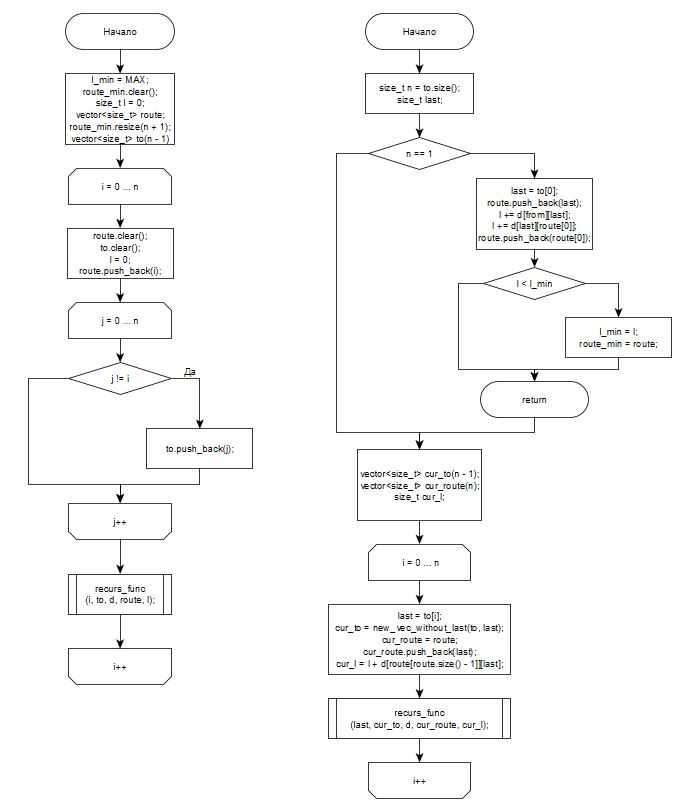
\includegraphics[scale=0.79]{1}
        		\caption{Схема алгоритма полного перебора}
        		\label{fig:def}
        	\end{center}
        \end{figure}

На рис. \ref{fig:def} представлена схема муравьиного алгоритма:
	\begin{figure}[h]
        	\begin{center}
        		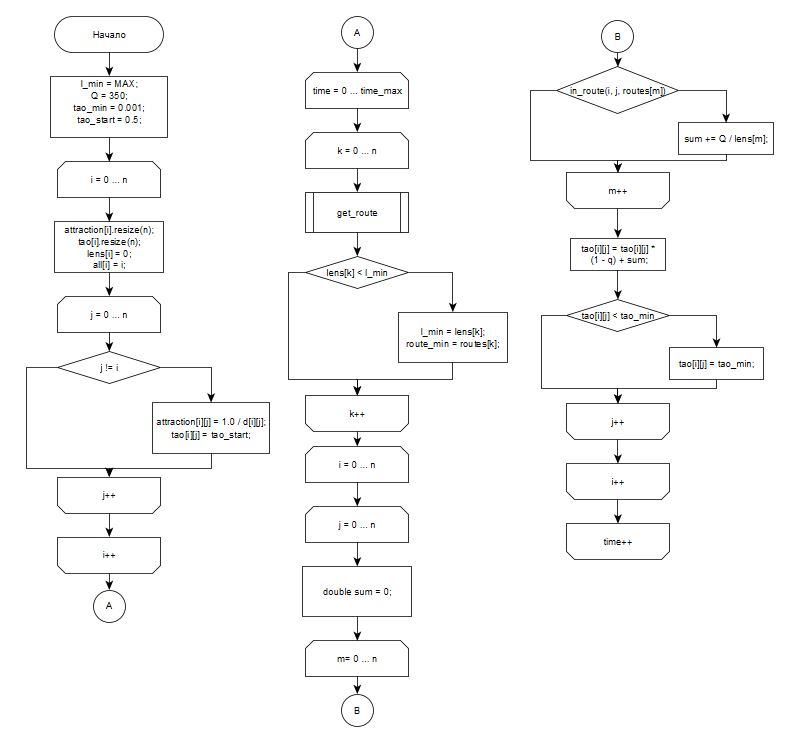
\includegraphics[scale=0.8]{2}
        		\caption{Схема муравьиного алгоритма}
        		\label{fig:def}
        	\end{center}
        \end{figure}

\chapter{Технологическая часть}
\section{Выбор ЯП}
Для реализации программ я выбрала язык программирования C++, так имею большой опыт работы с ним. Среда разработки - Visual Studio. \\

Для замера процессорного времени используется функция, возвращающая количество тиков (Листинг 3.1).\\

В листинге 3.2 рассмотрен алгоритм полного перебора, а в листинге 3.3 представлен муравьиный алгоритм.\\

\begin{lstlisting}[label=some-code,caption=Функция получения тиков]
unsigned __int64 tick() 
{ 
	return (__rdtsc()); 
}

\end{lstlisting}


\begin{lstlisting}[label=some-code,caption=Реализация полного перебора]
void recurs_func(size_t from, vector<size_t> to, vector<vector<size_t>> d, vector<size_t> route, size_t l) {

	size_t n = to.size();
	size_t last;
	if (n == 1) {
		last = to[0];
		route.push_back(last);
		l += d[from][last];
		l += d[last][route[0]];
		route.push_back(route[0]);
		if (l < l_min) {
			l_min = l;
			route_min = route;
		}
		return;
	}

	vector<size_t> cur_to(n - 1);
	vector<size_t> cur_route(n);
	size_t cur_l;
	for (size_t i = 0; i < n; i++) {
		last = to[i];
		cur_to = new_vec_without_last(to, last);
		cur_route = route;
		cur_route.push_back(last);
		cur_l = l + d[route[route.size() - 1]][last];
		recurs_func(last, cur_to, d, cur_route, cur_l);
	}

}

void perebor(size_t n, vector<vector<size_t>> d) {
	l_min = MAX;
	route_min.clear();
	size_t l = 0;
	vector<size_t> route;
	route_min.resize(n + 1);
	vector<size_t> to(n - 1);

	for (size_t i = 0; i < n; i++) {
		route.clear();
		to.clear();
		l = 0;

		route.push_back(i);
		for (size_t j = 0; j < n; j++)
			if (j != i)
				to.push_back(j);
		recurs_func(i, to, d, route, l);
	}

	cout << endl << "ROUTE: ";
	print_arr(route_min);
	cout << "LENGTH: " << l_min << endl << endl;
}

\end{lstlisting}


\begin{lstlisting}[label=some-code,caption=Реализация муравьиного алгоритма]
vector<double> get_probability(size_t from, vector<size_t> to, vector<vector<double>> tao, vector<vector<double>> attraction,
	size_t alpha, size_t beta) {

	double znam = 0, chisl = 0;
	size_t n = to.size();
	vector<double> result(n);
	for (size_t i = 0; i < n; i++) {
		znam += pow(tao[from][to[i]], alpha) * pow(attraction[from][to[i]], beta);
	}
	for (size_t j = 0; j < n; j++) {
		chisl = pow(tao[from][to[j]], alpha) * pow(attraction[from][to[j]], beta);
		result[j] = chisl / znam;
	}
	return result;
}

void get_route(vector<size_t> all, size_t start, vector<size_t> &route, size_t &len, vector<vector<size_t>> d,
	vector<vector<double>> tao, vector<vector<double>> attraction,
	size_t alpha, size_t beta) {

	route.resize(0);
	route.push_back(start);
	vector<size_t> to = new_vec_without_last(all, start);
	size_t n_1 = tao.size() - 2;
	size_t from;
	double coin, sum;
	bool flag;

	for (size_t i = 0; i < n_1; i++) {
		sum = 0;
		flag = true;
		from = route[i];
		vector<double> p = get_probability(from, to, tao, attraction, alpha, beta);
		coin = double(rand() % 10000) / 10000;
		for (size_t j = 0; j < p.size() && flag; j++) {
			sum += p[j];
			if (coin < sum) {
				route.push_back(to[j]);
				len += d[from][to[j]];
				to = new_vec_without_last(to, to[j]);
				flag = false;
			}
		}
	}
	len += d[route[route.size() - 1]][to[0]];
	route.push_back(to[0]);
	len += d[route[route.size() - 1]][route[0]];
	route.push_back(route[0]);
}

void ant(size_t n, vector<vector<size_t>> d, size_t alpha, size_t beta, double q, size_t time_max, ofstream& file) {

	l_min = MAX;
	route_min.clear();

	double tao_min, tao_start, Q;
	vector<size_t> all(n);
	Q = 350;
	tao_min = 0.001;
	tao_start = 0.5;

	vector<vector<size_t>> routes(n);
	vector<size_t> lens(n);

	vector<vector<double>> attraction(n);
	vector<vector<double>> tao(n);

	for (size_t i = 0; i < n; i++) {
		attraction[i].resize(n);
		tao[i].resize(n);
		lens[i] = 0;
		all[i] = i;
		for (size_t j = 0; j < n; j++) {
			if (i != j) {
				attraction[i][j] = 1.0 / d[i][j];
				tao[i][j] = tao_start;
			}
		}
	}

	for (size_t time = 0; time < time_max; time++) {
		for (size_t k = 0; k < n; k++) {
			get_route(all, k, routes[k], lens[k], d, tao, attraction, alpha, beta);
			if (lens[k] < l_min) {
				l_min = lens[k];
				route_min = routes[k];
			}
		}
		for (size_t i = 0; i < n; i++)
			for (size_t j = 0; j < n; j++) {
				double sum = 0;
				for (size_t m = 0; m < n; m++) {
					if (in_route(i, j, routes[m]))
						sum += Q / lens[m];
				}

				tao[i][j] = tao[i][j] * (1 - q) + sum;
				if (tao[i][j] < tao_min)
					tao[i][j] = tao_min;
			}
	}
}

\end{lstlisting}



\chapter{Исследовательская часть}

\section{Постановка эксперимента}

Был проведен сравнительный анализ реализаций муравьиного алгоритма и полного перебора. Замеры времени проводились для графов с количеством вершин от 2 до 10 с шагом 1. Значения коэффциентов составили $\alpha$ = 0, $t_{max}$ = 5, $\rho$ = 0.1.\\
С результатами можно ознакомиться в таблице 4.1:\\

\begin{table}[H]
	\caption{Результаты рамеров времени для алгоритма полного перебора и муравьиного алгоритма}
	\begin{center}
		\begin{tabular}{|c|c|c|}
			\hline
			Количество вершин &Полный перебор& Муравьиный алгоритм \\\hline
			2&0.00005&0.0002\\
			3&0.0002&0.0007\\
			4&0.0005&0.0011\\
			5&0.002&0.0017\\
			6&0.01&0.002\\
			7&0.06&0.003\\
			8&0.54&0.005\\
			9&5.65&0.008\\
			10&59.3&0.02\\
			\hline
		\end{tabular}
	\end{center}
\end{table} 




\begin{center}
\begin{tikzpicture}
	\begin{axis}[
		    xlabel={Разница времени выполнения частей конвейера},
		    ylabel={Время в милисекундах},
		    xmin = 0, xmax = 10,
		    ymin = 0, ymax = 60,
		    legend pos=north west,
		    ymajorgrids=true,
		    grid style=dashed,
		]
		\legend{ 
	        Алгоритм полного перебора,
	        Муравьиный алгоритм
	        }
  		\addplot[
  		    color=blue,
  		    mark=square,
  		    ]
  		    coordinates {
  		    (2,  0.00005)
  		    (3,  0.0002)
  		    (4, 0.0005)
  		    (5, 0.002)
			(6, 0.01)
			(7, 0.06)
			(8, 0.54)
			(9, 5.65)
			(10, 59.3)
  		    };
  		\addplot[
  		    color=red,
  		    mark=square,
  		    ]
  		    coordinates {
  		     (2,  0.0002)
  		    (3,  0.0007)
  		    (4, 0.0011)
  		    (5, 0.0017)
			(6, 0.002)
			(7, 0.003)
			(8, 0.005)
			(9, 0.008)
			(10, 0.02)
  		    };
		\end{axis}
	\end{tikzpicture}
	\end{center}
       
\section{Параметризация муравьиного алгоритма на основании проведенного эксперимента}	

Для различных значений параметров $\alpha$, $\beta$, $\rho$ и $t_{max}$ для каждой из нескольких матриц смежности с помощью муравьиного алгоритма и перебора была найдена некоторая длина маршрута. Далее выбраны наилучшие сочетания параметров муравьиного алгоритма на этих данных.\\
Параметр $\alpha$ менялся от 0 до 10, параметр $\rho$ менялся от 0.1 до 0.9, параметр $t_{max}$ менялся от 5 до 100.\\
Итого были выявлены оптимальные сочетания параметров (представлены в таблице 4.2):\\

\begin{table}[H]
	\caption{Результаты решения задачи параметризации}
	\begin{center}
		
	\begin{tabular}{|c|c|c|c|}
		\hline
		$\alpha$ &$\beta$ & $\rho$ & $t_{max}$ \\\hline
		4&6&0.6&20\\
		6&4&0.3&40\\
		 1&9&0.7&50\\
		 6&4&0.9&70\\
		 3&7&0.6&80\\
		 6&4&0.25&90\\
		 \hline
	\end{tabular}
\end{center}
\end{table} 
\
 

\section{Вывод}

Муравьиный алгоритм при количестве вершин больше 5 выигрывает во времени выполнения у алгоритма полного перебора, так как не смотря на то, что на 2-5 вершинах перебор выигрывает, его время выполнения очень быстро растет при увеличении числа вершин.\\

Также, для заданного класса данных были найдены параметры, которые обеспечивают наиболее оптимальное решение.\\



\chapter*{Заключение}
\addcontentsline{toc}{chapter}{Заключение}
В ходе работы был изучен и реализован оригинальный муравьиный алгоритм, а также простой перебор. Были получены наиболее оптимальные параметры для быстрого и правильного решения задачи коммивояжера на матрице из десяти "городов".




\end{document}